\documentclass[border=10pt]{standalone}
\usepackage{pgfplots}
\usepgfplotslibrary{fillbetween}
\pgfplotsset{compat=1.18}
\begin{document}
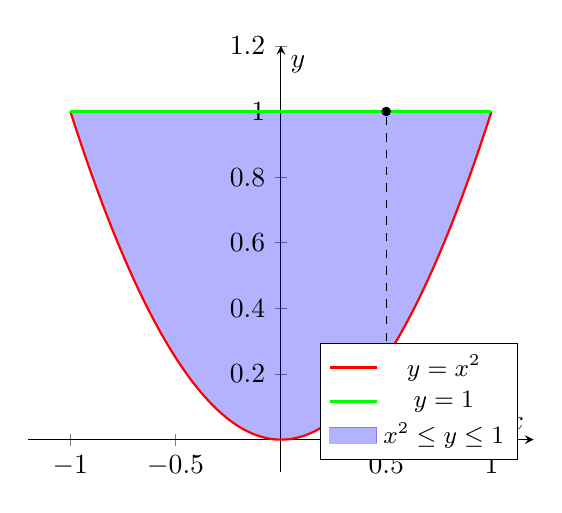
\begin{tikzpicture}
\begin{axis}[
    axis lines=middle,
    xlabel={$x$}, ylabel={$y$},
    xmin=-1.2, xmax=1.2, ymin=-0.1, ymax=1.2,
    domain=-1:1, samples=200,
    width=8cm, height=7cm,
    legend pos=south east,
    legend style={font=\small},
]
\addplot[name path=A, red, thick] {x^2};
\addlegendentry{$y=x^2$}
\addplot[name path=B, green, thick] {1};
\addlegendentry{$y=1$}
\addplot[blue, opacity=0.3] fill between[of=A and B];
\addlegendentry{$x^2\le y\le1$}
\draw[dashed] (axis cs:0.5,0.25) -- (axis cs:0.5,1);
\filldraw (axis cs:0.5,0.25) circle (1.5pt);
\filldraw (axis cs:0.5,1) circle (1.5pt);
\end{axis}
\end{tikzpicture}
\end{document}